\chapter{Sviluppo}
\label{chap:development}
In questo capitolo verranno descritte le motivazioni della scelta del linguaggio e come sono state implementate le varie componenti del servizio.
\section{Scelta dei linguaggi}
Durante questa fase sono stati analizzati i possibili linguaggi da utilizzare per la ricostruzione del servizio.

\subsection{Backend}
Per rispettare i requisiti del problema (vedi \cref{sec:limitazioni}) è stato scelto \texttt{Go} come linguaggio per la riscrittura dei servizi di upstream e downstream.
La scelta è stata presa secondo i seguenti criteri:

\begin{itemize}
    \item \textbf{Compilazione nativa}: a differenza dei linguaggi usati in precedenza (\texttt{PhP} e \texttt{python}), Go è un linguaggio compilato. Questo permette di ottenere un file binario eseguibile nativamente dal sistema operativo, senza la necessità di un interprete o di una macchina virtuale a runtime, con conseguenti vantaggi in termini di prestazioni e tempi di avvio del servizio.
    
    \item \textbf{Binari statici}: a differenza di \texttt{C} e \texttt{C++}, i binari prodotti dal compilatore di Go sono file statici, ovvero includono al loro interno tutte le librerie necessarie all'esecuzione. Questo elimina la dipendenza da librerie condivise installate sul sistema (\emph{dependency hell}) e semplifica notevolmente il dispiegamento del servizio, rendendolo particolarmente adatto a essere containerizzato (ad esempio tramite immagini Docker minimali basate su \texttt{scratch} o \texttt{alpine}) e distribuito su ambienti eterogenei senza dover gestire l'installazione di un runtime specifico.
    
    \item \textbf{Concorrenza nativa}: Go supporta in maniera nativa la gestione di routine parallele leggere, le cosiddette \emph{goroutine}, gestite direttamente dal runtime del linguaggio con un overhead significativamente inferiore rispetto ai thread tradizionali del sistema operativo. Il linguaggio fornisce inoltre una struttura dati apposita, il \emph{canale} (\texttt{chan}), che consente la comunicazione e la sincronizzazione sicura tra goroutine. Questo aspetto è risultato fondamentale per lo sviluppo dell'upstream aggregator, che necessitana di gestire in maniera concorrente ed efficiente numerosi flussi di dati provenienti dal servizio di downstream.
    
    \item \textbf{Gestione automatica della memoria}: pur essendo un linguaggio compilato con prestazioni vicine a quelle di \texttt{C}/\texttt{C++}, Go integra un \emph{garbage collector}, riducendo la complessità di sviluppo e il rischio di errori tipici della gestione manuale della memoria.
    
    \item \textbf{Libreria standard e semplicità}: Go dispone di una libreria standard ricca, in particolare per quanto riguarda la gestione di rete e protocolli \ac{HTTP}, elemento centrale per lo sviluppo di servizi di upstream e downstream. La sintassi minimale e le scelte di design orientate alla leggibilità riducono inoltre la curva di apprendimento e favoriscono la manutenibilità del codice nel tempo.
\end{itemize}

\subsection{Integrazione con FlashStart 2026}
A differenza dei servizi di backend l'integrazione con il nuovo applicativo non è stata necessaria una analisi per la scelta dei linguaggi.
Sono stati infatti utilizzati \texttt{typescript} per l'interazione tra l'applicazione il servizio backend e \texttt{NodeJs} con \texttt{react} per la creazione dell'interfaccia grafica, in allineamento con le scelte conseguite dall'azienda ospitante.

\section{Wrapper ICMP}
L'esecuzione del ping sul server è l'operazione più importante del sistema.
La versione legacy del software eseguiva semplicemente il comando \texttt{ping -c MAX\_PING network}\sidenote{\texttt{MAX\_PING} è una variabile che indica quanti pacchetti \ac{ICMP} inviare per l'esecuzione del ping} con una conseguente normalizzazione del risultato.
Come analizzato nel in precedenza (vedi \cref{section:downstream}) il parser si basa sulla manipolazione di una stringa con indici di riga fissi; Questo rende il sistema molto fragile ad errori, una piccola variazione nel formato del risultato del comando potrebbe causare il fallimento della richiesta.

\lstinputlisting[
    float,
    language=go,
    label={lst:icmp-wrapper},
    caption={[Implementazione della funzione di invio del messaggio echo.] L'invio avviene in maniera trasparente rispetto alla versione del protocollo \ac{IP} utilizzato attraverso l'utilizzo del pattern strategy discusso in precedenza (\Cref{sec:ipversion-handler}).}
    ]{listings/echoWrapper.go}

Il nuovo sistema è stato creato con l'affidabilità alla base.
Al posto di eseguire una shell bash, è stata utilizzata la libreria di Go (\texttt{golang.org/x/net/icmp}) per eseguire chiamate \ac{ICMP} \cite{rfc792} attraverso la rete; A questa libreria è stato creato un wrapper che permetta l'utilizzo facilitato di una libreria altrimenti notevolmente complessa.

Il wrapper permette di inviare una serie di messaggi \ac{ICMP} \texttt{Echo} con id univoci in modo da filtrare pacchetti non inviati dal sistema (\Cref{lst:icmp-wrapper}).
Attraverso il pattern strategy definito in precedenza, è in grado di inviare in maniera trasparente la richiesta sia su una rete IPv4 che su una rete IPv6, in base all'indirizzo fornito dall'utente. Infine permette opzionalmente la possibilità di impostare il \ac{TTL} ad ogni pacchetto.
Quest'ultima feature permette una potenziale futura espansione del servizio attuale con l'aggiunta del traceroute.

Questo wrapper risolve il problema della fragilità del risultato, poiché il parsing del risultato non viene più fatto in base all'output di un comando di una bash. Il risultato finale viene calcolato sulla base dei risultati di ogni pacchetto che vengono salvati in locale.
\section{Bounded Parallelism}
Il linguaggio Go mette a disposizione due costrutti nativi per la gestione di routine concorrenti: le ``goroutine'' e i ``canali'' (\texttt{chan}) strutture dati in grado di gestire automaticamente la concorrenza senza provocare race conditions.
I canali possono essere usati per implementare un comportamento simile a quello dei semafori nella programmazione concorrente, e sono lo strumento principale di Go per la sincronizzazione e la comunicazione tra goroutine.



L'implementazione del bounded concurrency pattern si è basata da una funzione che calcola il \emph{checksum MD5} di tutti i file in una directory specificata \cite{ajmani2014pipelines}, riadattandola secondo le necessità del sistema in sviluppo.

\lstinputlisting[
    float,
    language=go,
    label={lst:server-walker},
    caption={[Implementazione della funzione addressWalker.] La funzione \texttt{serverListWalk} inizializza la goroutine che avrà il compito di erogare uno ad uno gli indirizzi dei vari server della rete sul canale di distribuzione.}
    ]{listings/addressWalker.go}

\begin{figure}
    \centering
    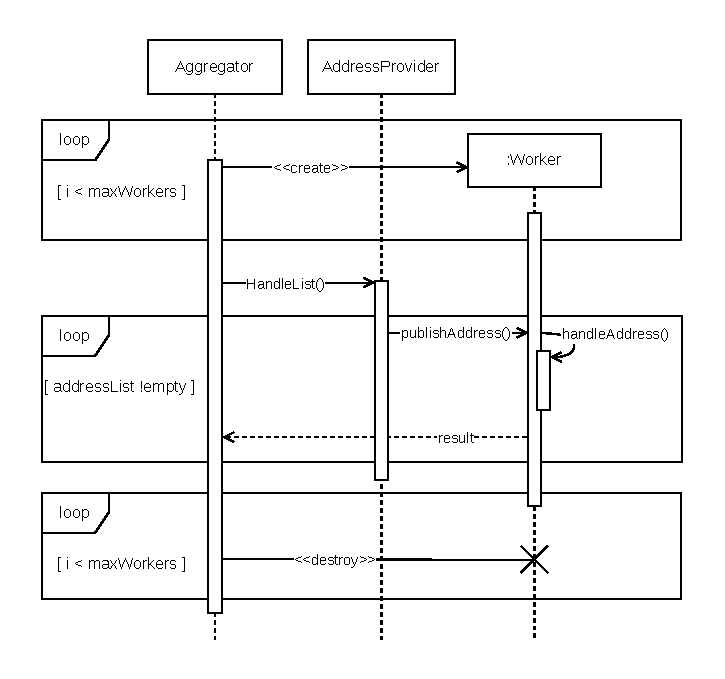
\includegraphics[width=.8\linewidth]{figures/bounded-concurrency-go.pdf}
    \caption[Esecuzione della funzione di aggregazione.]{Diagramma di sequenza della funzione di aggregazione, dalla creazione dei thread worker fino alla loro distruzione.}
    \label{fig:bounded-concurrency-go}
\end{figure}

Il funzionamento illustrato in figura \cref{fig:bounded-concurrency-go} si basa su tre canali distinti:
\begin{itemize}
    \item \emph{Canale di distribuzione degli indirizzi}: eroga uno alla volta ciascun indirizzo dei server da interrogare. Canale utilizzato dalla funzione \texttt{serverListWalk} (\Cref{lst:server-walker})  e sul quale si mettono in ascolto i nodi worker.
    \item \emph{Canale di raccolta dei risultati}: eseguito dal thread principale colleziona i risultati calcolati da ciascun thread worker.
    \item Un canale utilizzato per la segnalazione della conclusione del processo.
\end{itemize}

\lstinputlisting[
    float,
    language=go,
    label={lst:worker-node},
    caption={[Implementazione del thread worker.] Il thread worker ascolta il canale di distribuzione degli indirizzi. Al ricevimento di un \ac{IP} interroga il relativo server e ritorna il risultato ottenuto per poi rimettersi in ascolto sul canale.}
    ]{listings/workerNode.go}

Una volta inizializzati i canali viene creato l'insieme di lavoratori, la cui implementazione è riportata nel \cref{lst:worker-node} che eseguiranno le richieste di latenza ai vari server.

Questa implementazione permette un effettivo parallelismo a runtime solamente se il sistema sottostante ha una CPU multicore e se la variabile \texttt{GOMAXPROCS}\footnote{\texttt{GOMAXPROCS} è la variabile che indica il numero massimo di thread che si possono usare per eseguire goroutines in parallelo.} lo permette \cite{michealcarlos2025gomaxproc}.

Dalla versione 1.24 in poi di go la variabile assume di default il numero totale di CPU cores nella macchina.
\section{Frontend}
Per lo sviluppo del frontend è stato coinvolto un esperto di user experience, con l'obiettivo di mantenere un elevato standard di usabilità e garantire coerenza di stile con il resto dell'applicativo. Questo coinvolgimento ha permesso di affrontare la progettazione non solo dal punto di vista funzionale, ma anche tenendo conto dei principi di design consolidati, evitando così di introdurre incoerenze visive o pattern di interazione poco intuitivi per l'utente finale.

La progettazione è partita dall'analisi del design della vecchia pagina, individuando punti di forza e criticità dell'interfaccia esistente. L'obiettivo della nuova versione era quello di riproporre le stesse funzionalità in maniera più chiara e pulita, semplificando la fruizione delle informazioni senza però stravolgere le abitudini d'uso già acquisite dagli utenti. La figura~\ref{fig:wireframe} illustra il design generale che si intendeva riprodurre, evidenziando la disposizione degli elementi principali e il flusso di interazione previsto.
\begin{figure}
    \centering
    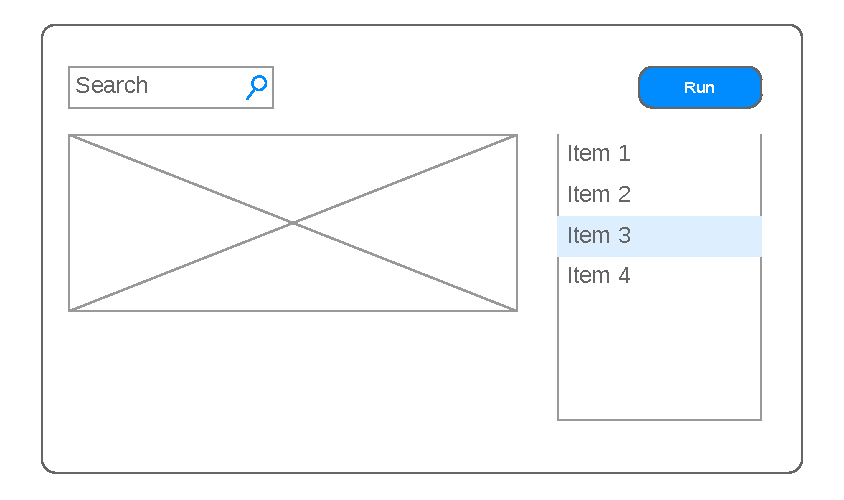
\includegraphics[width=1\linewidth]{figures/ui-wireframe.pdf}
    \caption[Wireframe dell'interfaccia utente]{Struttura generale delle informazioni da trasmettere attraverso l'interfaccia obiettivo, realizzata sulla base della struttura della piattaforma legacy.}
    \label{fig:wireframe}
\end{figure}

Inizialmente è stato proposto un design semplice, che riproponeva sostanzialmente la struttura della pagina precedente, limitandosi a modificarne lo stile grafico per renderlo più moderno e in linea con gli standard visivi attuali. Questa prima iterazione illustrata in figura \cref{fig:intermediate-design}, pur rappresentando un miglioramento estetico, non introduceva sostanziali cambiamenti nella disposizione dei contenuti né nell'esperienza d'uso complessiva.

\begin{figure}
    \centering
    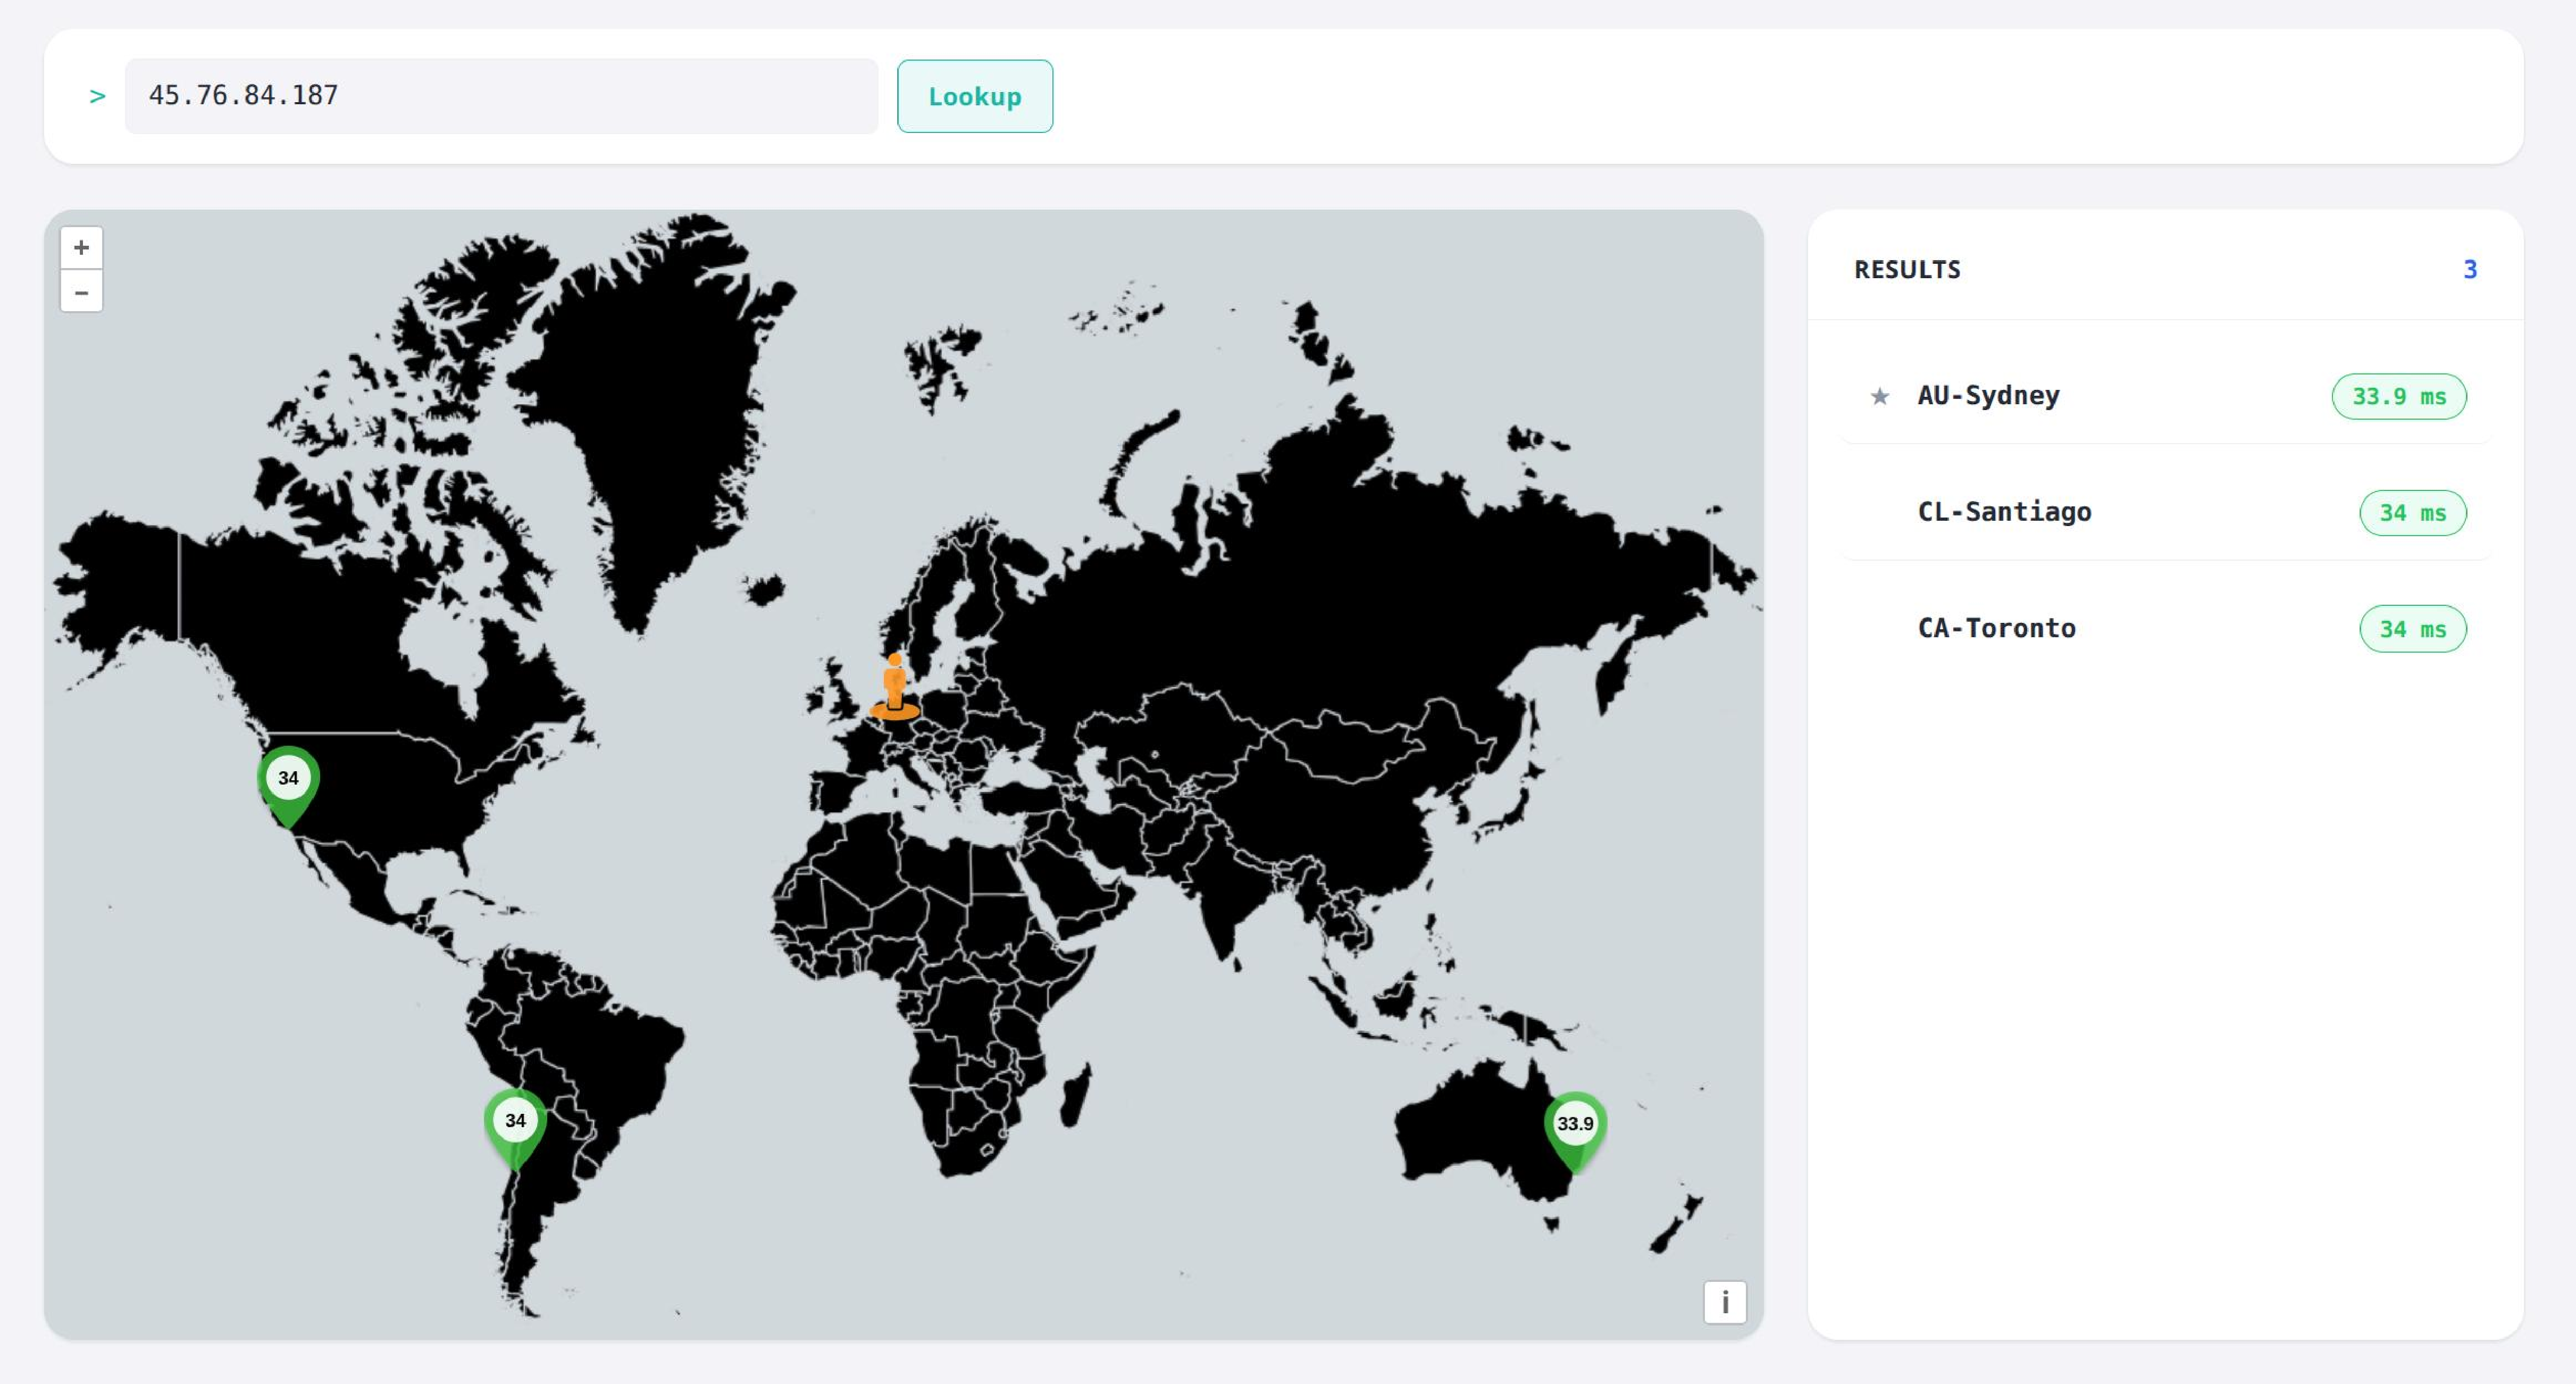
\includegraphics[width=1\linewidth]{figures/intermediate-design.pdf}
    \caption[Primo redesign dell'interfaccia]{Primo redesign dell'interfaccia, con un semplice restyling grafico della piattaforma legacy.}
    \label{fig:intermediate-design}
\end{figure}


Dopo l'intervento dell'esperto UX, il mockup si è evoluto significativamente: da un lato mantenendo coerente lo stile visivo con il resto della piattaforma FlashStart 2026, dall'altro introducendo una struttura più flessibile e modulare, pensata per accogliere eventuali evoluzioni future senza richiedere una riprogettazione radicale dell'interfaccia. Questo processo iterativo, frutto di diversi cicli di revisione e confronto, ha portato alla definizione del design finale mostrato in figura~\ref{fig:final-mockup}.

\begin{figure}
    \centering
    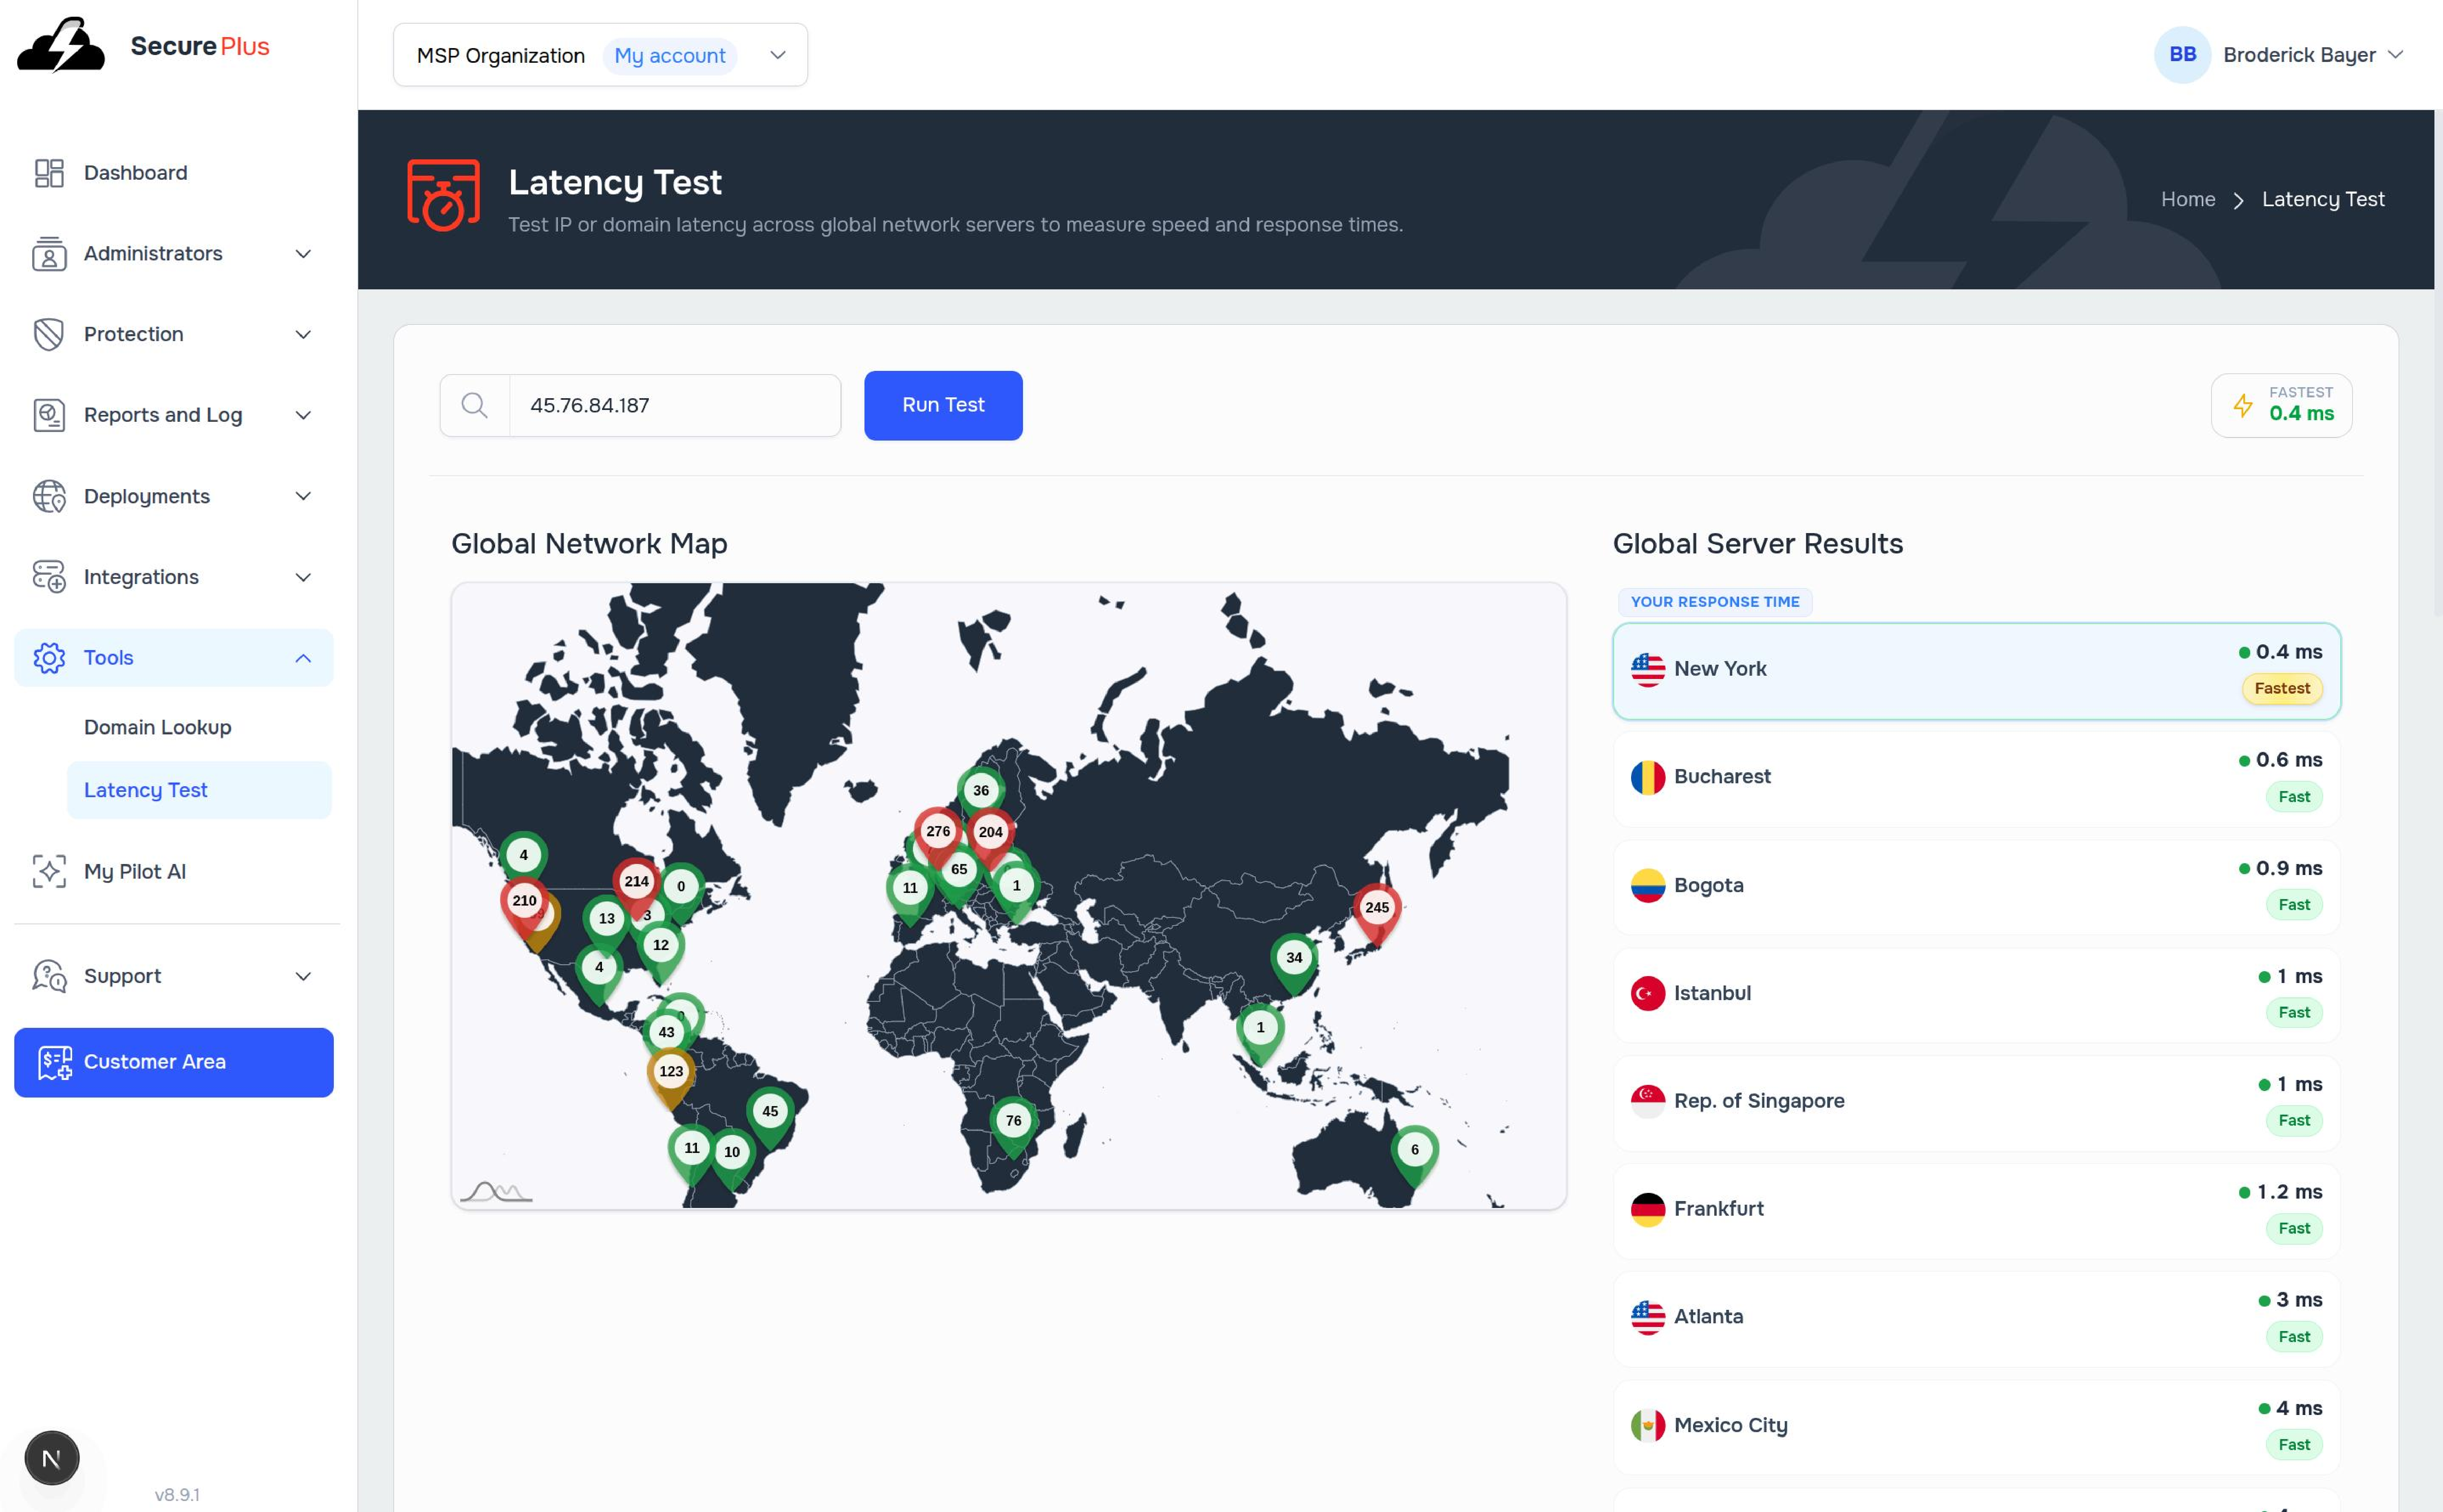
\includegraphics[width=1\linewidth]{figures/final-design.pdf}
    \caption[Design finale]{Design finale dell'interfaccia utente, adottato nella versione rilasciata.}
    \label{fig:final-mockup}
\end{figure}


Il design finale mostra i dati in maniera chiara e organizzata, con uno stile riadattato per integrarsi con il resto dell'applicazione. Oltre a migliorare la leggibilità e l'immediatezza delle informazioni presentate, la nuova struttura lascia spazio a possibili estensioni future, consentendo l'aggiunta di nuove funzionalità o sezioni senza compromettere la coerenza complessiva dell'interfaccia.
\subsection{Scelta della libreria per la mappa}
La scelta della libreria per il rendering della mappa è stata un processo lungo e articolato, durante il quale sono stati analizzati pro e contro di diverse soluzioni tecnologiche, valutando in particolare il compromesso tra prestazioni, costi e complessità di manutenzione.

Inizialmente è stata analizzata \texttt{OpenLayers}, una libreria open source pensata per il rendering ad alte prestazioni di mappe dinamiche all'interno di applicazioni web. La libreria consente di visualizzare la mappa del mondo suddividendola in ``tile''\footnote{Una tile è una sezione quadrata della mappa corrispondente a un certo livello di zoom.}, un approccio che massimizza le prestazioni e garantisce fluidità durante le operazioni di spostamento e zoom, poiché vengono caricate solo le porzioni di mappa effettivamente visibili all'utente.

Tuttavia, per renderizzare una mappa basata su tile è necessario appoggiarsi a un map provider in grado di rispondere alle richieste delle singole tile generate dal client. Dopo numerose ricerche, sono emerse due opzioni percorribili:
\begin{itemize}
    \item \emph{Provider a pagamento}: sottoscrivere un abbonamento mensile a un servizio esterno che fornisce le \ac{API} necessarie per il recupero delle singole tile. Questa opzione è stata scartata per evitare di introdurre dei costi ricorrenti.
    \item \emph{Self hosting}: allestire un server dedicato contenente l'intero set di tile ed esporre autonomamente le \ac{API} necessarie. Anche questa strada è stata scartata, poiché l'insieme completo delle immagini richiedeva oltre 100 Gb di spazio di archiviazione, un requisito ritenuto eccessivo rispetto alle risorse disponibili per il progetto.
\end{itemize}

Un'ulteriore alternativa valutata è stata quella di renderizzare l'intera mappa come una singola immagine vettoriale. Questo approccio avrebbe eliminato la dipendenza da provider esterni e da grandi quantità di storage, ma si è rivelato inadeguato dal punto di vista delle prestazioni: il rendering di un'unica geometria vettoriale complessa comportava tempi di caricamento elevati e una scarsa reattività, rendendo l'esperienza utente poco fluida.

Considerati i limiti delle soluzioni precedenti, è stata infine scelta una seconda libreria: \texttt{amcharts5}, una libreria generica per la creazione di grafici che offre, tra i propri moduli, anche il supporto al rendering di mappe dinamiche. L'utilizzo di questa libreria si è rivelato un buon compromesso tra le prestazioni desiderate e la gratuità del servizio: non richiede infatti alcun provider esterno per le tile, poiché si basa su geometrie vettoriali ottimizzate, garantendo al contempo un livello di interattività e fluidità adeguato alle esigenze del progetto.